\begin{comment}
2.1.3 Management Summary und Web-Publikation
Das Management Summary soll 2-5 Seiten umfassen sowie eine bis zwei Figuren enthalten. Es richtet sich an den „gebildete Laien“ auf dem Gebiet und beschreibt daher in erster Linie die (neuen und eigenen) Ergebnisse und Resultate der Arbeit. Die Sprache soll knapp, klar und stark untergliedert sein.
Grundlage für das Management Summary kann der Broschüren-Eintrag sein, den die Abteilung bei Diplomarbeiten jeweils früh verlangt, um eine Broschüre zu drucken. Das Management Summary dient als Vorlage für eine allfällige Web-Publikation.
Das Abstract und das Management Summary werden - zeitlich gesehen - gegen Schluss der Arbeit geschrieben und bilden zusammen mit den Schlussfolgerungen im technischen Bericht den am häufigsten gelesenen Teil der Arbeit. Diese Dokumente sollen daher am Sorgfältigsten ausgearbeitet sein.
Die folgenden Stichworte sollen die typische Struktur illustrieren, wobei die genaue Ausführung jeweils auf die spezifischen Bedürfnisse und Randbedingungen eines Projekts anzupassen ist. Diese Struktur kann auch für die Präsentation der Arbeit als "Richtschnur" dienen.
1. Ausgangslage
Warum machen wir das Projekt?
Welche Ziele wurden gesteckt (Kann-Ziele, Muss-Ziele)
Was machen andere / welche ähnlichen Arbeiten gibt es zum Thema?
Vorgehen: Was wurde gemacht? In welchen Teilschritten?
Risiken der Arbeit?
Wer war involviert (Durchführung, Entscheide usw.)?
Was konnte von anderen verwendet werden?
2. Ergebnisse
Was ist das Resultat?
Bewertung der Resultate, was ist Neuartig an der Arbeit?
Zielerreichung bezüglich Kann-/Muss-Zielen
Abweichungen (positiv und negativ) und kurze Begründung dafür
(Externe) Kosten der Arbeit?
Was ist der Nutzen (quantifizierbar/nicht quantifizierbar)?
3. Ausblick
Was hat man mit Durchführung des Projekts gelernt?
Verbleibende Probleme, (zukünftige) Gegenmassnahmen bez. Risiken
Was würde man anders machen, was ist weiter zu tun

Überschriften (Unterkapitel) ohne Nummerierung einsetzen!
\end{comment}


\phantomsection
\addcontentsline{toc}{chapter}{Management Summary}

\chapter*{Management Summary}
\glsresetall

\section*{Ausgangslage}

\gls{nine} betreibt über 1500 Linux-Serversysteme mit unterschiedlichen Konfigurationen. Die Software-Komponenten werden über herkömmliche Debian-Pakete installiert. Bei der Veröffentlichung von Sicherheitsupdates müssen diese zeitnah auf sämtlichen betroffenen Serversystemen installiert werden, was bisher manuell mit verschiedenen Bash-Scripts erreicht wird.

Dies hat mehrere Nachteile: Es gibt keine zuverlässigen Feedback-Mechanismen, verursacht jede Woche mehrere Stunden Aufwand und resultiert im schlimmsten Fall in einer Verzögerung von mehreren Tagen bis zur Installation.

\begin{figure}
  \centering
    \includegraphics[width=0.6\textwidth]{upd89-overview-before}
  \caption{Ausgangslage: Ein Mitarbeiter aktualisiert jedes System einzeln}
  \label{fig:overview-before}
\end{figure}

\section*{Vorgehen und Technologien}

Der Kunde gab vor, dass auf jedem Server ein Agent laufen muss, der ausstehende Updates an ein Kontrollcenter meldet, welches mit Ruby on Rails und PostgreSQL umgesetzt wird. So kann das System leicht in die bestehende Umgebung eingebunden und weiterentwickelt werden. 

Auf dem Agent wird eine Python-Bibliothek zur Anbindung an die Debian-Paketverwaltung verwendet. Die Kommunikation zwischen Agenten und Kontrollcenter erfolgt per HTTPS mit Clientzertifikaten, um eine sichere Kommunikation auch über unsichere Netze zu gewährleisten.

\begin{figure}
  \centering
    \includegraphics[width=0.6\textwidth]{upd89-overview}
  \caption{Die Lösung ermöglicht das zentrale Updatemanagement einer grossen Anzahl von Servern.}
  \label{fig:overview}
\end{figure}

\section*{Ergebnisse}   

Im Rahmen dieser Bachelorarbeit wurde eine Open-Source-Lösung entwickelt, welche das Einspielen von Updates auf Serversystemen vereinfacht. Der Benutzer kann über die Software bestimmen, auf welchen Systemen welche Updates durchgeführt werden sollen. Diese werden an die entsprechenden Systeme gesendet, dort automatisch ausgeführt und zurück an das Kontrollcenter gemeldet.


Der Benutzer kann zudem Systeme und Pakete gruppieren, um Masseninstallationen von Updates auf mehreren Systemen gleichzeitig durchzuführen. Durch verschiedene Auswertungen kann er sich eine bessere Übersicht über die Systeme und Pakete verschaffen.

\begin{figure}
  \centering
    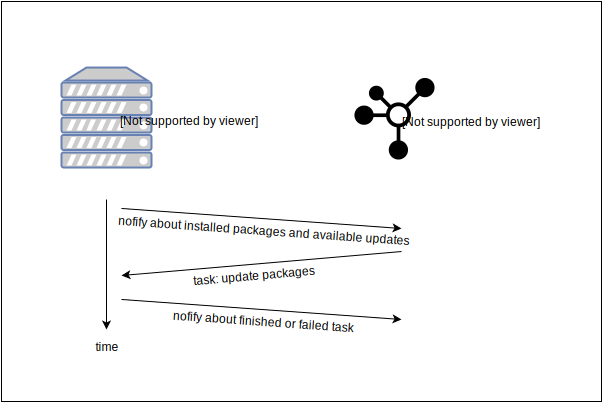
\includegraphics[width=0.6\textwidth]{upd89-processes}
  \caption{Die asynchrone Kommunikation erfolgt ereignisgesteuert.}
  \label{fig:processes}
\end{figure}

\section*{Ausblick}

Die Software wurde mit dem Ziel entwickelt, als Open-Source-Lösung veröffentlicht zu werden. Deshalb ist der Quellcode offen erhältlich und das Benutzen oder Erweitern der Applikation ist erwünscht. \gls{nine} wird die Software für ihre Zwecke noch erweitern und in ihre bestehende IT-Landschaft einbetten.

Eine Anbindung an andere Paketverwaltungssysteme ist denkbar, da die Agents nur über eine API mit dem Kontrollcenter kommunizieren und die Implementation der Agents unabhängig davon ist.

\begin{figure}
  \centering
    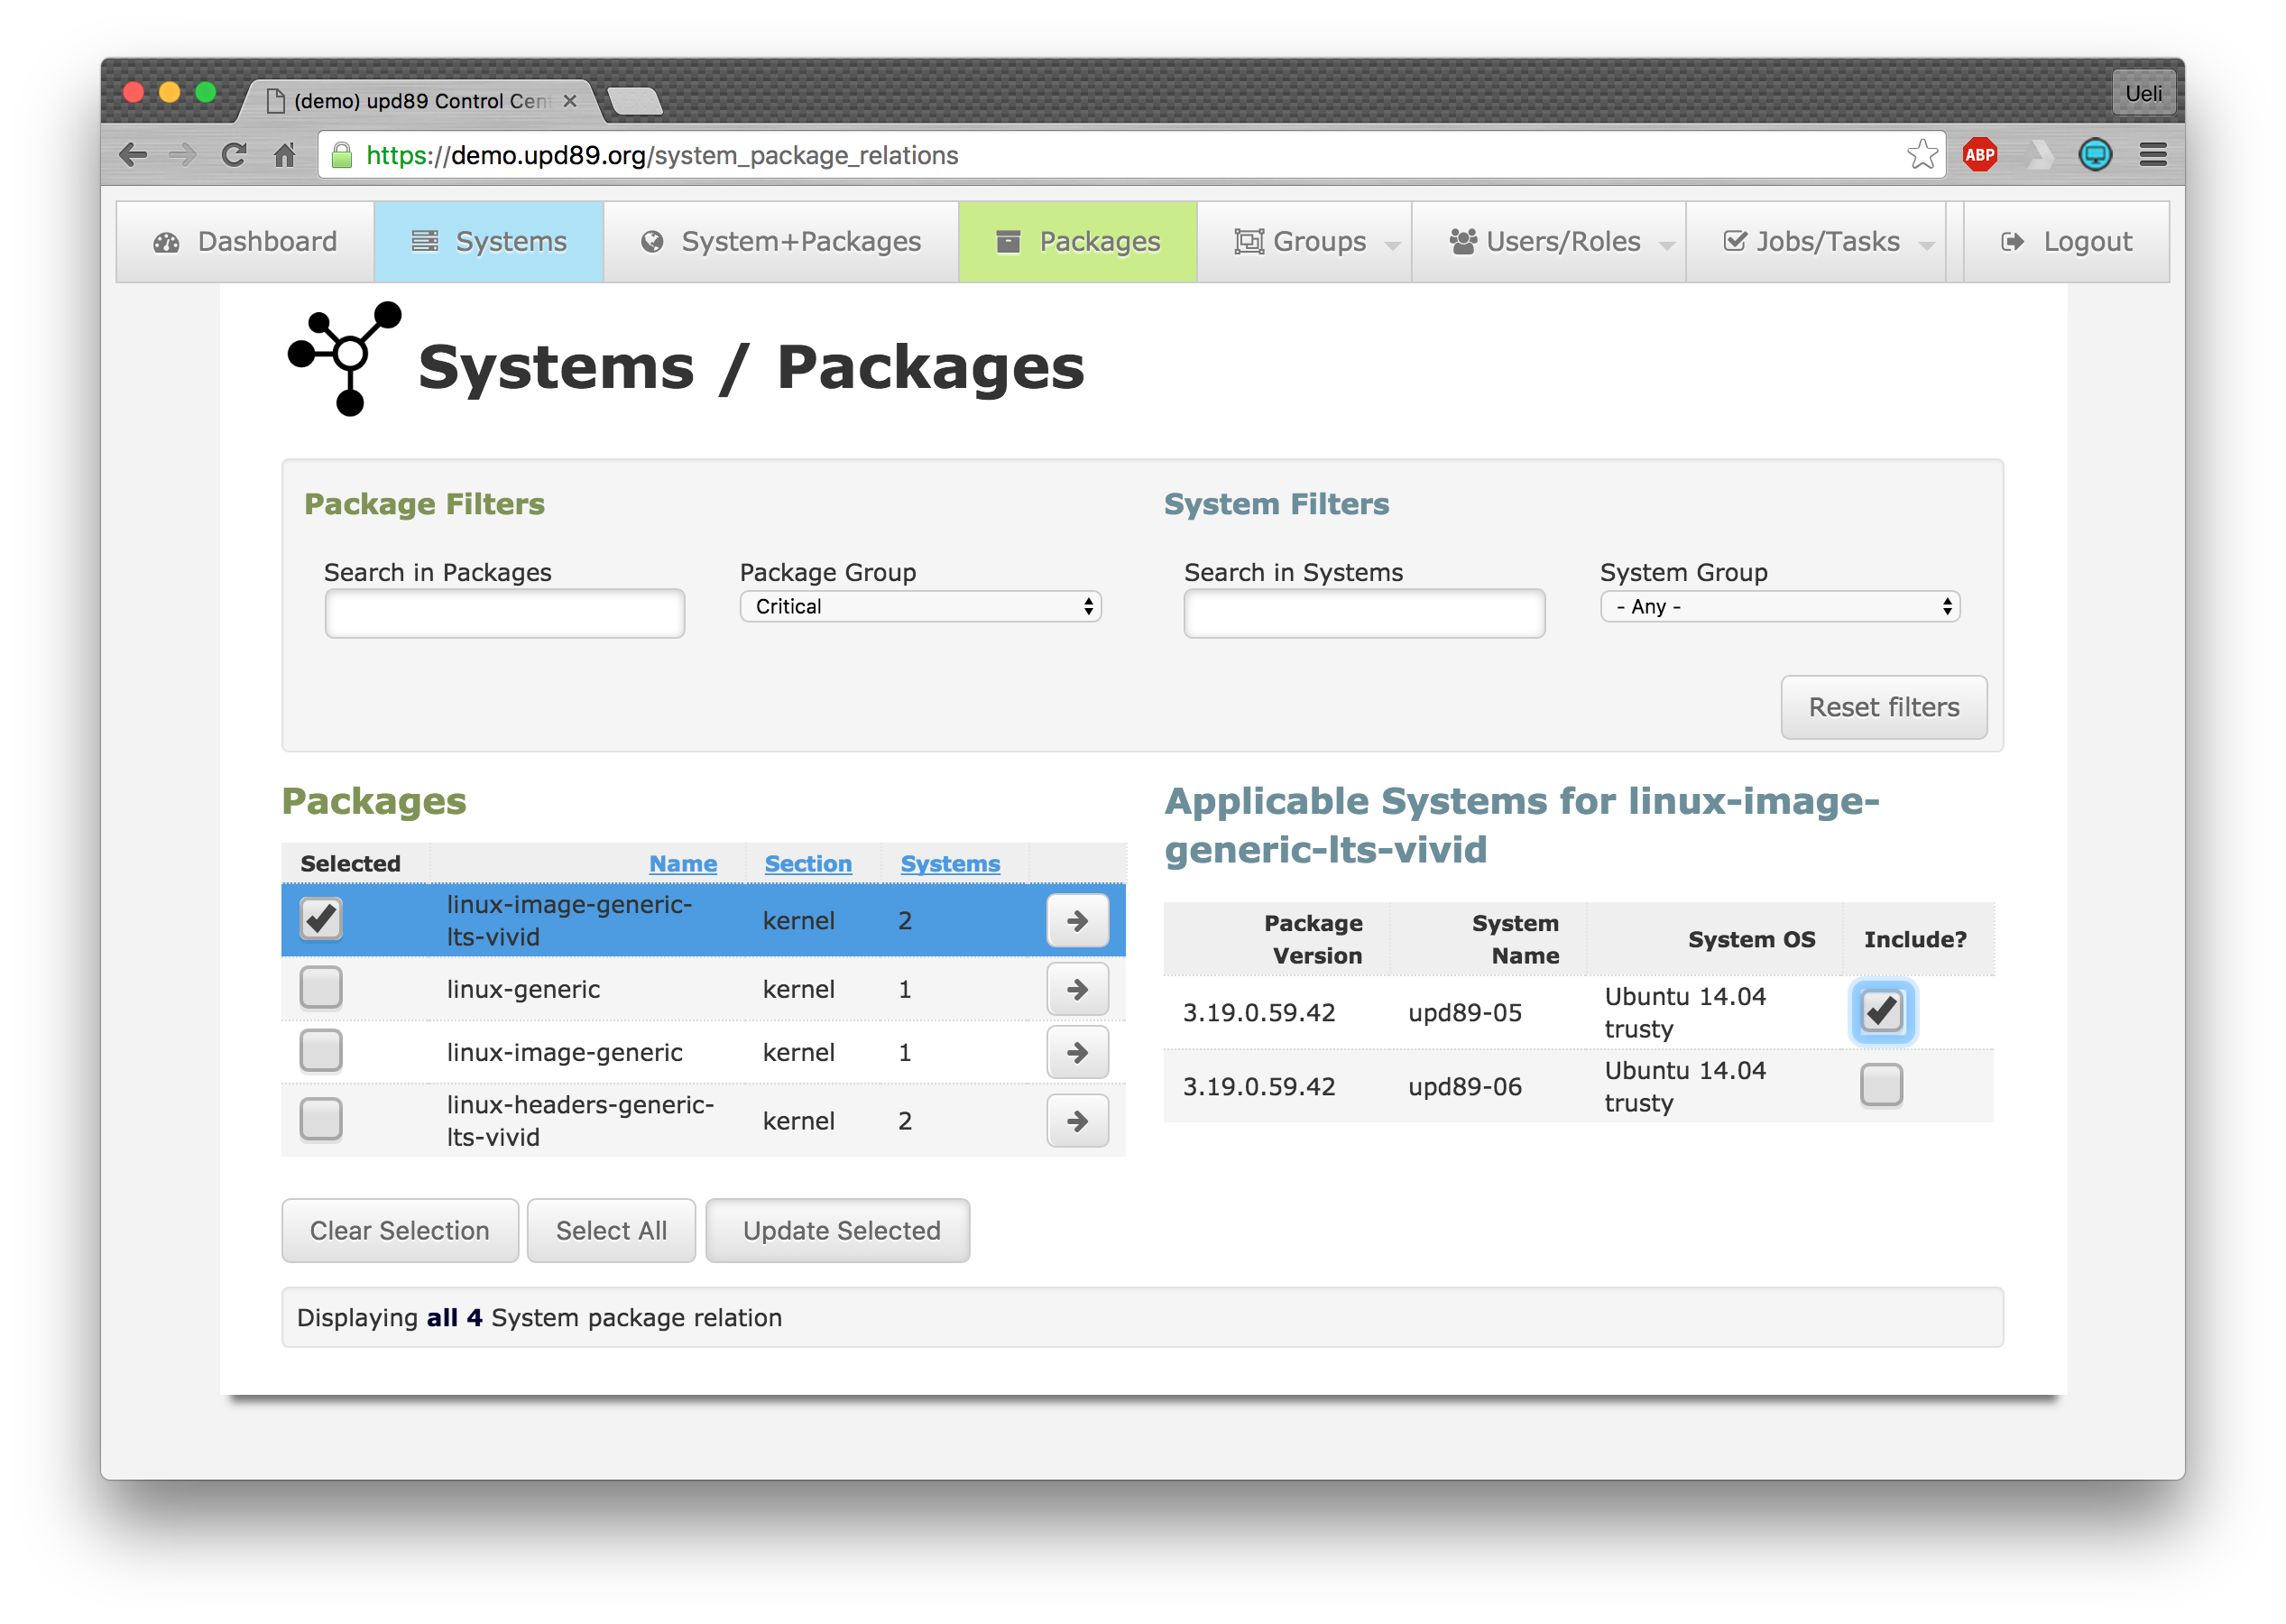
\includegraphics[width=0.8\textwidth]{screenshot_comboview}
  \caption{Die Weboberfläche ermöglicht die gezielte Auswahl von Updates.}
  \label{fig:userinterface}
\end{figure}